\chapter{System Design}
\label{chapter:system_design}

\section{Core Design Decisions}
  The \acrshort{DDE} Framework, created as a result of this thesis, is designed to be distributed in nature with the concept of Actor Programming~[\autoref{sec:actorProgramming}]. It provides an inherently distributed nature to applications built on top of it. The \acrshort{DDE} framework itself is built using the concept of ‘message-passing’~[\autoref{sec:messagePassing}] to alleviate any possibility of concurrency issues, making \acrshort{DDE} applications thread-safe.

  The framework is based on the following principles:
\begin{itemize}
  \item All messages sent by the framework are based on the ‘fire and forget’ concept.
  \item The framework does not guarantee the delivery of messages.
  \item A message is delivered at most once.
  \item For simplicity, consistency and persistence, a message is always routed through a Message Queuing System~[\autoref{subsec:mqs}], even though a target isolate may belong to the same isolate system in the same logical or physical node.
  \item Dequeuing a message (from a MQS) by a worker isolate is based on a pull mechanism, not a push mechanism.
%  \item Exceptions thrown at child isolates are handled by ‘spawner’ of that isolate. Hence, implementing the idea of supervision and “let it crash” ideology~[\autoref{subsec:letItCrash}].
\end{itemize}

\section{The Framework}
\begin{figure}[H]
  \centering
  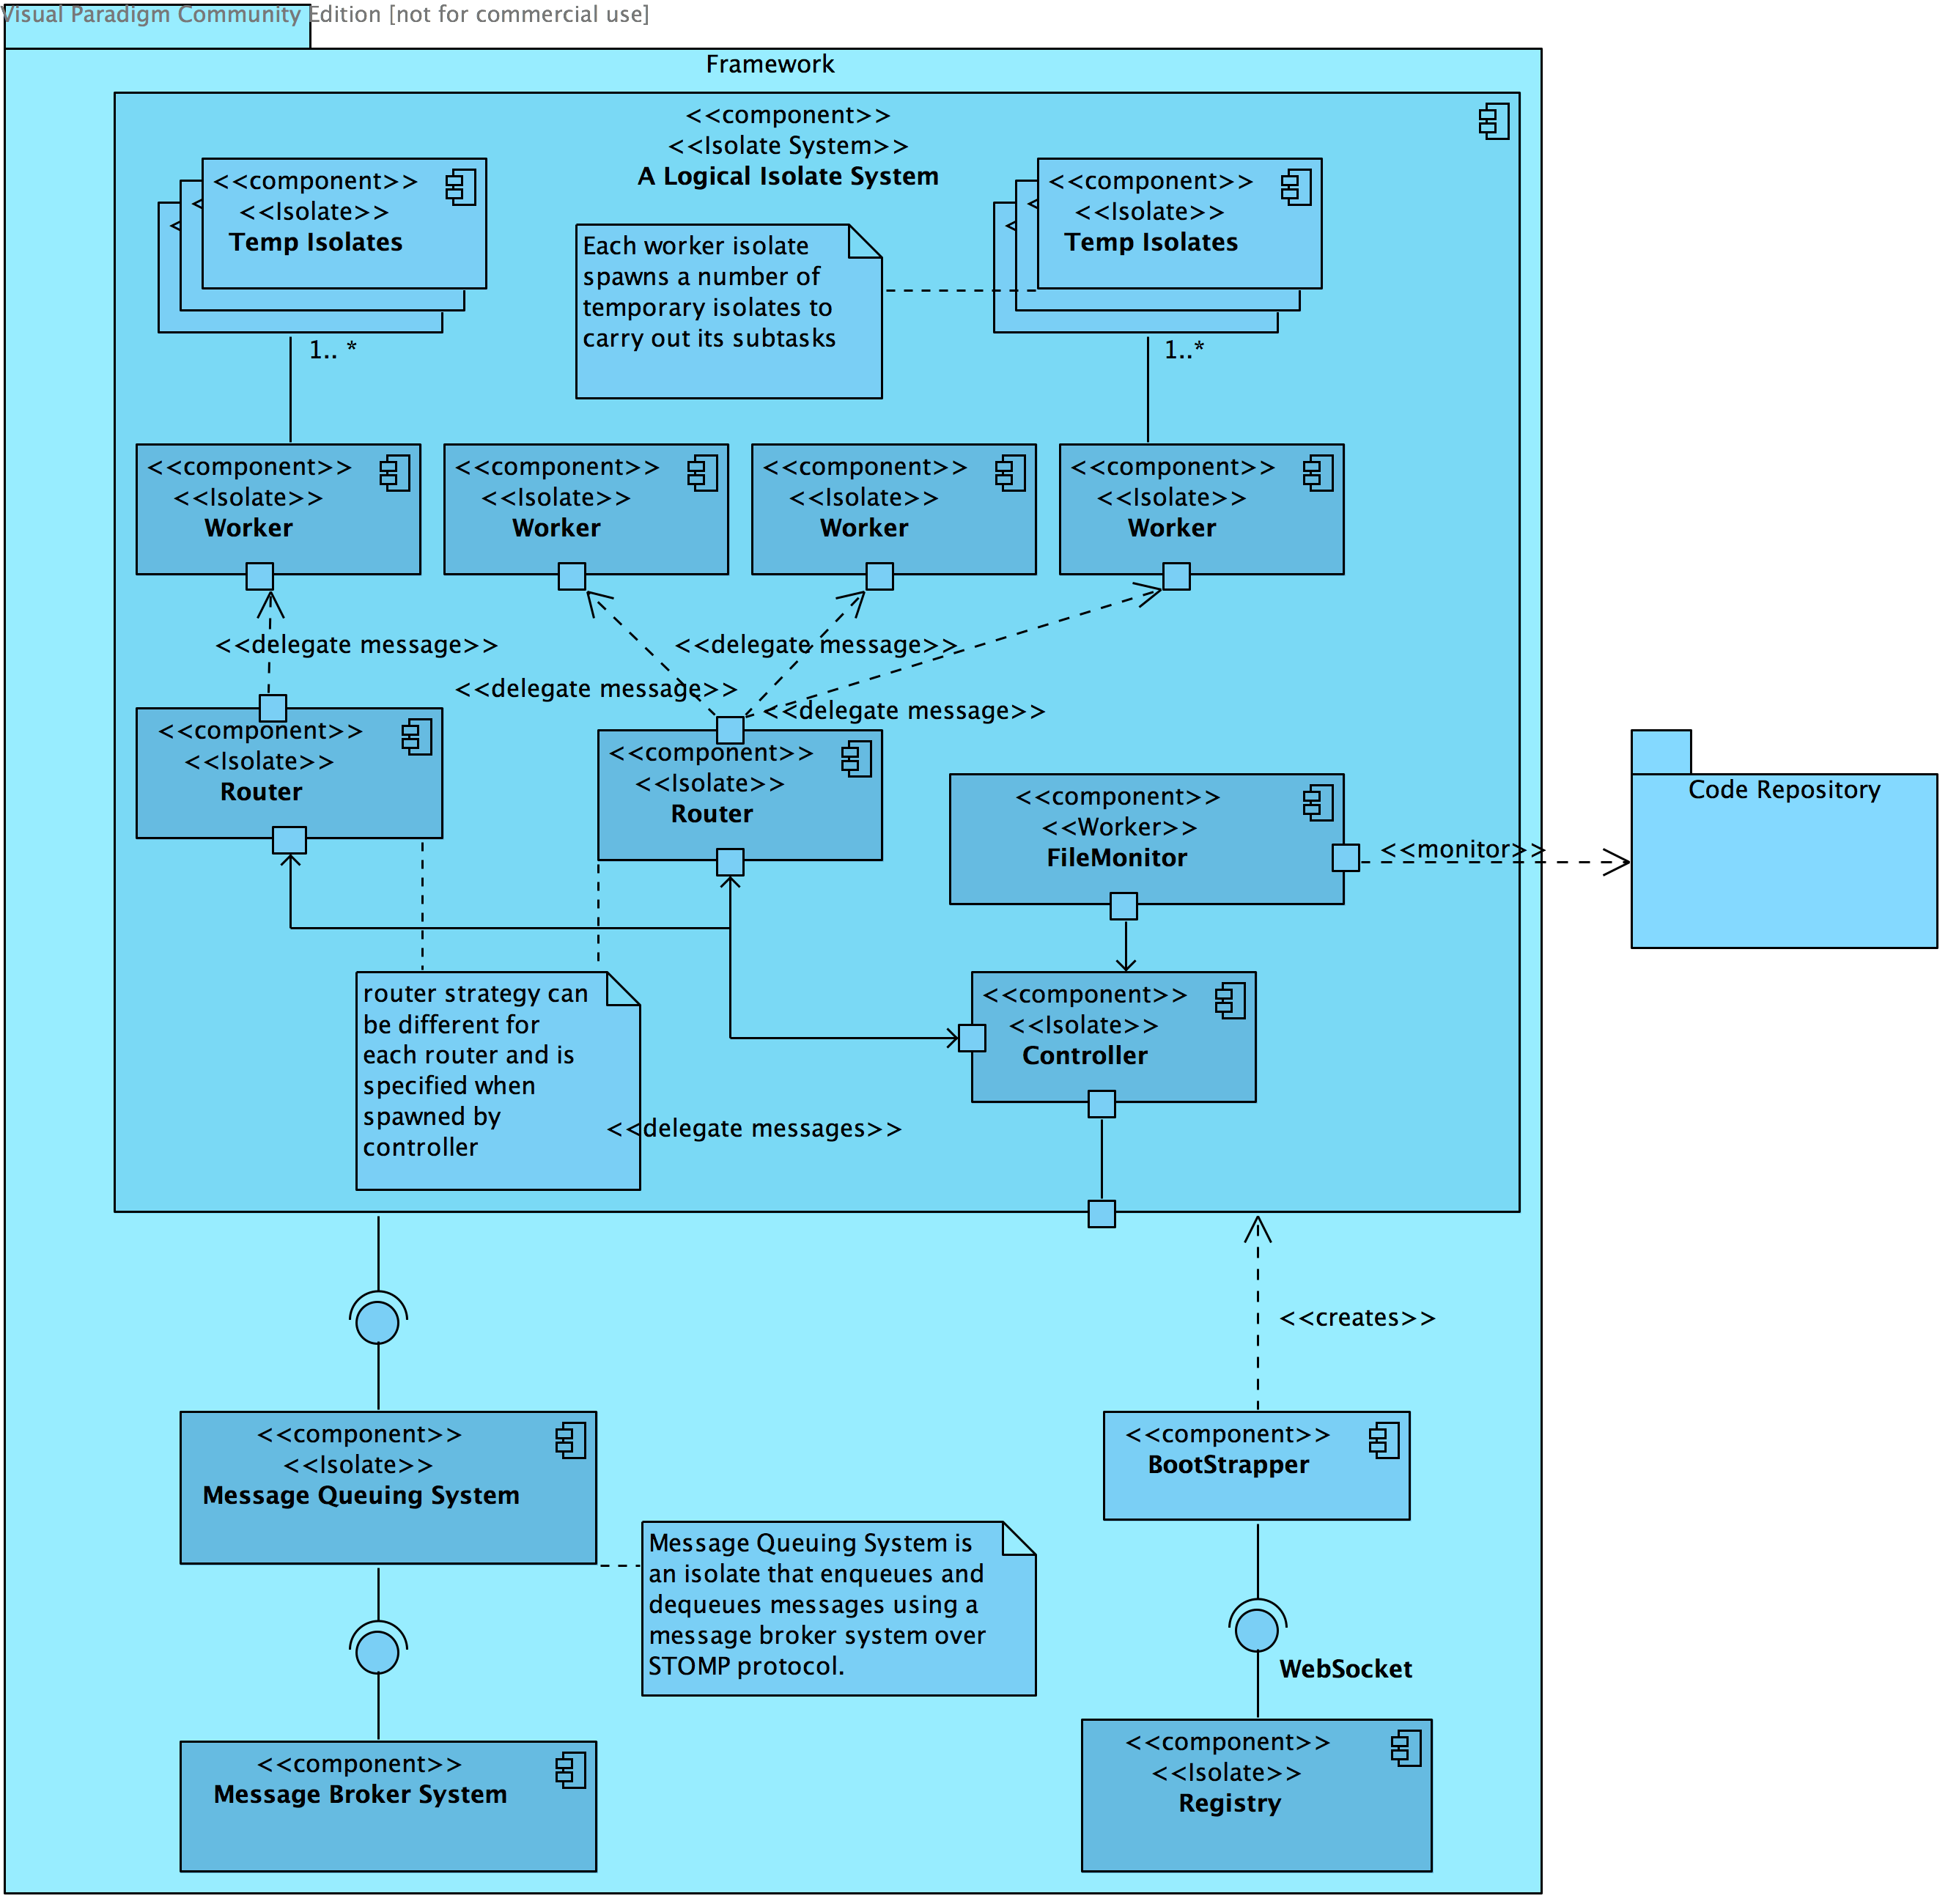
\includegraphics[width=1\textwidth]{figures/componentDiagram}
  \caption[Architecture of the framework]{Architecture of the framework}
  \label{fig:architecture}
\end{figure}

The \acrshort{DDE} framework is comprised of an ‘Isolate System’, a ‘Registry’, a ‘Message Queuing System’, a ‘Message Broker System’ and an ‘Activator’. \autoref{fig:architecture} depicts the major components and sub-components of the framework.

  \subsection{Isolate System}
  \label{sub:isolate-system}
  An isolate system is analogous to an actor system~\autoref{subsec:actorSystem}. Just as an actor system consists of a group of actors working together, an isolate system consists of a group of ‘Worker’ isolates. It consists of different hierarchies which form an organization-like structure. The bottom most entities are ‘Worker’ isolates, which are managed by a ‘Router’. Routers are managed by the ‘Controller’ and the controller is spawned by a top level isolate.

  Each isolate system has a unique id, which is a \acrshort{uuid}. It is generated when an isolate system is bootstrapped. For bootstrapping, an isolate system needs the WebSocket address of a Message Queuing System, and a ‘name’ for itself. The name is simply an alias and it should not be confused with the unique id. Another isolate system with the same name may exist in other nodes but a unique id is exclusive for a particular instance of an isolate system.

  A ‘Bootstrapper’ in a physical node can start up several isolate systems. But, a logical isolate system is not limited to a single physical node. The ‘Worker’ isolates of an isolate system can be distributed across several systems.

  Bootstrapping of an isolate system includes: generating a new unique id, opening up a ‘ReceivePort’, and connecting to a ‘Message Queuing System’. After opening up a ‘ReceivePort’, the isolate system starts listening on that port for messages so that it can receive incoming messages from the ‘Controller’. If a connection with the MQS fails or disconnects, the isolate system retries at a regular interval to establish a connection. Since the connection to the MQS takes place asynchronously, the isolate system moves forward and spawns the controller regardless of the establishment of connection to the MQS.

  \subsubsection{Adding Worker Isolates to an Isolate System}
  As an isolate system is a top level isolate, it spawns a controller. A controller spawns one or several routers and each router spawns worker isolates. \autoref{fig:addIsolateSequence} shows a message flow sequence in different components while starting up an isolate system and deploying a worker isolate in it.

  \begin{figure}[H]
    \centering
    \tiny
  \begin{sequencediagram}
  \newinst[0.5]{u}{Developer}
  \newinst[0.5]{reg}{Registry}
  \newinst[0.5]{b}{Bootstrapper}
  \newinst[0.5]{s}{Isolate System}
  \newinst[0.5]{c}{Controller}
  \newinst[0.5]{r}{Router}
  \newinst[0.5]{w}{Worker}

    \mess{b}{connect and register}{reg}
    \mess{u}{deploy isolate}{reg}
    \mess{reg}{initialize isolate system}{b}
    \mess{reg}{add isolate}{b}
    \mess{s}{spawn controller}{c}
    \mess{c}{SendPort}{s}

    \begin{call}{b}{addIsolate()}{s}{}
    \end{call}
    \mess{s}{add isolate}{c}
    \mess{c}{spawn router}{r}
    \mess{r}{SendPort}{c}

    \mess{r}{spawn worker}{w}
    \mess{w}{SendPort}{r}

  \end{sequencediagram}
    \caption{Adding a Worker isolate to an isolate system}
  \end{figure}
  \label{fig:addIsolateSequence}
  \normalsize

  An isolate system is initialized without any Workers running in it. The Workers are added with an appropriate load balancer after the isolate system is initialized. The \emph{addIsolate} method starts up worker isolates in the isolate system. The method has the following required and optional arguments:
  \begin{description}
    \item{\itshape{name}} \textendash{} A name for a pool of isolates. A deployed isolate has its own name but overall the name is concatenated with the name of the isolate system to denote the hierarchy. For instance, an isolate with the name ‘account’ becomes ‘bank/account’ where ‘bank’ is the name of the isolate system.
    \item{\itshape{sourceUri}} \textendash{} Location of the source code from which the isolate shall be spawned. The path may either be an absolute path to a local file system or a full http or https URI.
    \item{\itshape{workersPaths}} \textendash{} List of destinations where each of the isolates should be spawned. To spawn a worker isolate locally, ‘localhost’ should be used as the path, and to spawn in a remote node, a WebSocket path like “ws://192.168.2.9:42042/activator” should be used. The number of isolates that should be spawned is determined by the length of this list. If multiple copies of isolates should be spawned in a node, the location can be repeated. For instance [“localhost”, “localhost”] results in spawning of two identical isolates in the local machine which is load balanced by the specified router.
    \item{\itshape{routerType}} \textendash{} Type of load balancing technique that one would like to use to effectively distribute incoming messages. By default, the \acrshort{DDE} framework provides three types of routers: Round-Robin, Random and Broadcast. It is also possible to use a custom router implementation by extending the \emph{Router} class of the framework. A custom router can be loaded by providing an absolute path (either file or http/https URI) for the source code location.
    \item{\itshape{hotDeployment}} \textendash{} This argument is optional and defaults to ‘true’. Setting it to ‘true’ enables continuous monitoring of source code. If any change in the source code is identified, instances of isolates spawned by this \emph{addIsolate} function in the current isolate system are restarted, without redeploying the whole system.
    \item{\itshape{args}} \textendash{} Custom additional arguments to be passed into each isolate instance during spawning. This argument is also optional and can be safely ignored.
  \end{description}

  \subsubsection{Message Handling in a Top Level Isolate}
  Typically, a message in an isolate system may arrive from three sources: the Message Queuing System via a WebSocket, the Controller via a ReceivePort or the Bootstrapper via direct method invocation. As Dart is a single threaded programming language~[\autoref{sec:isolates}], only one message is handled at a time by the top level isolate.

  A Message Queuing System sends the data over a WebSocket in JSON string format, which should be deserialized to the ‘Map’ data type before further processing. As a received message contains a queue name from which it is dequeued, the name of the queue is parsed and transformed to the name and address of the corresponding isolate. The message is then forwarded to the Controller that this instance of the isolate system has spawned.

  Messages arriving from a controller are either dequeue requests or messages for enqueuing (that should be sent to the Message Queuing System). Dequeue requests are sent from isolates that have completed a task and are ready to accept another message. For dequeue requests, the sender of the message is identified to determine the corresponding name of the queue. Then the dequeue request is forwarded to the MQS via an open WebSocket port. For messages that should be delivered to another isolate, the name of the target isolate is used to determine the name of the queue and then sent to the MQS for enqueuing.

Messages arriving from the bootstrapper are either KILL messages or messages to get isolate details. A request to get detailed information of an isolate system and its isolates are made via web interface or RESTful web services of the registry~[\autoref{subsec:registry}]. When such requests are made, the registry forwards them to the respective bootstrapper~[\autoref{subsubsec:bootstrapper}]. The bootstrapper then invokes a function provided by the top level isolate. Then, the top level isolate sends a message to a controller to get the list of isolates the controller is managing and waits asynchronously for a future reply. As soon as a response is received from the controller, the top level isolate sends the response to the bootstrapper as a return value of the invoked function.

  Another type of message is a ‘KILL’ message, which is used to terminate a worker isolate. Since a top level isolate does not directly manage running worker isolates, the message is forwarded to the controller which is next in the hierarchy. Similarly, when the ‘KILL’ message is sent to an isolate system to shut it down, the top level isolate forwards the KILL message to its controller and closes all open ports including WebSocket ports and ReceivePorts. After that it waits for the VM garbage collector to clean up the memory reserved by it.

  \subsubsection{Controller}
  Every isolate system has a single controller which is spawned by the top level isolate of an isolate system. A controller stays idle until it receives a message to spawn an isolate. After receiving a spawn message, the controller spawns and manages routers in an isolate system. It also spawns a ‘FileMonitor’ for each ‘hot deployment’ feature enabled router. When a RESTART message is received from a FileMonitor, the controller sends a RESTART\textunderscore{}ALL message to the designated router, and the router restarts all worker isolates it has spawned.

  A controller is also responsible for replying to the request for the list of isolates in an isolate system. It achieves this by keeping a detailed record of each router and number of worker isolates each router is handling. The list gets updated as soon as a worker isolate is killed or a new worker isolate is added.

  As a controller is the ‘spawner’ of routers and the ‘spawnee’ of the top level isolate, it forwards messages as well as dequeue requests coming from routers to the top level isolate.

  \subsubsection{Router}
  \label{subsubsec:router}
  A router is spawned by a controller. The router creates and is responsible for a group of workers which are instances of the same class. Since an isolate is single threaded, creation of multiple instances of an isolate is desirable for concurrency. When a message arrives in a router from a controller, the router, based on its defined routing policy, delegates the message to one of the worker isolates. The routing policy may be chosen at the time of deployment of a worker isolate.

  A router uses a routing policy to distribute messages among the group of isolates it is handling. The default routing policies that are available in the framework are listed in \autoref{tab:routers}
\begin{table}[htsb]
  \caption[Routing techniques provided by the framework]{List of routing techniques provided by the framework}\label{tab:routers}
  \centering
  \begin{tabular}{l l}
    \toprule
      \bf{Router} & \bf{Description} \\
    \midrule
      Round Robin & Messages are passed in round-robin fashion to its \\ & worker isolates.\\
      Random & Randomly picks one of its worker isolates and sends\\ & the message to that Worker isolate.\\
      Broadcast & Replicates and sends message to all of its Worker isolates.\\
    \bottomrule
  \end{tabular}
\end{table}

    In addition to the available routing policies of the framework, it is also possible to add a new routing technique by simply extending the ‘Router’ class, which requires the \emph{selectWorker} function to be implemented. The overridden \emph{selectWorker} function may either return a list of workers or a single worker. The ability to implement a custom router opens up possibilities for numerous load balancing techniques. For instance, a simple multicasting router that replicates a message only to the workers that are spawned locally can be implemented easily by selecting such workers using their deployment paths and returning them as a ‘List’.

    As a router manages the worker isolates it has spawned, it is responsible for effectively terminating and restarting the worker isolates. It also buffers messages that arrive when the worker isolates are not ready. This usually occurs during the creation and restarting of worker isolates.

    If a router does not receive any message from a worker for a certain amount of time, the router sends a PING message to check if the worker isolate is alive and ready to accept more messages. If the worker isolate responds with a PONG message the router sends a dequeue request to the controller. This mechanism is present in the framework to prevent starvation of worker isolates. Starvation is caused when a dequeue message that may have been sent earlier does not reach the Message Queuing System due to a network issue or unavailability of the MQS.

  \subsubsection{Worker}
  \label{subsubsec:worker}
  The ‘Worker’ of the framework is an abstract class, which should be extended by the class that a developer of \acrshort{DDE} applications creates. The worker unwraps messages that arrive from the router and retrieves the headers. ‘sender’ and ‘replyTo’ headers of messages are extracted before forwarding them to the worker instance. By unwrapping the messages that are encapsulated by various headers, the abstract Worker class makes sure that the messages are delivered to the target implementation of the Worker isolate immutated and in intended form.

  To extend a ‘Worker’ isolate, one must implement the \emph{onReceive} function which handles incoming messages and carries out application logic tasks. If a task is complex, a developer may divide it into subtasks and spawn temporary isolates to carry out those subtasks concurrently. Temporary isolates may be terminated once their subtask has been carried out.

  \emph{send}, \emph{reply} and \emph{ask} are helper functions provided by the abstract Worker class to send a message to another worker isolate. These functions automatically add the sender and receiver headers to messages that are sent.

  \paragraph{Sending a Message}
  \label{para:sendMessage}
  To send a message from one worker isolate to another, the framework provides the \emph{send} function. It requires the ‘message’ and ‘address’ of a target worker isolate as its arguments. A reply path can be optionally set, so that the replied message is sent to a different worker isolate for further processing. The named parameter\footnote{Dart's named parameter is an optional argument in the function} ‘replyTo’ should be used to set the address of the intended recipient of the reply message; eg:
\begin{lstlisting}[numbers=none]
  send("A simple text message", "demosystem/printer");
\end{lstlisting}

\begin{lstlisting}[numbers=none]
  send("Another message", "demosystem/jsonConverter", replyTo: "demosystem/printer");
\end{lstlisting}

  \paragraph{Asking For a Reply}
  \label{subsec:askMessage}
  Sometimes a worker isolate might need a reply from another isolate for further processing or before replying to the sender of a message. In such case, the worker isolate specifically asks the target isolate to reply to this particular instance of the worker isolate.

  A sample use case of ‘ask’ may be a worker isolate maintaining a connection with a browser via HTTP. In this case, as the port cannot be serialized and passed to other isolates as messages, another instance of the same worker will not be able to respond to the request made in that connection.

  Similar to the \emph{send} function, the \emph{ask} function takes the ‘message’ and ‘address’ of a target worker isolate as its arguments; eg:
\begin{lstlisting}[numbers=none]
  ask("current time", "demosystem/timeKeeper");
\end{lstlisting}
  \paragraph{Replying to a Message}
  \label{subsec:replyMessage}

  To reply to a message the framework provides the \emph{reply} function. It expects only a single ‘message’ argument because the response is sent to the worker isolate specified by the sender. The \emph{reply} function can be used to respond to any message; eg:
\begin{lstlisting}[numbers=none]
  reply("Current time is: $time");
\end{lstlisting}

  \subsubsection{Proxy}
  A ‘Proxy’ is a special type of a worker isolate. When a worker isolate should be spawned in a remote node, a router instead spawns a proxy isolate in a local node. Once the Proxy isolate is created, it connects to the ‘Isolate Deployer’~[\autoref{subsubsec:isolateDeployer}] of the remote node. After establishing a WebSocket connection with the Isolate Deployer, the proxy isolate forwards the request to spawn the worker isolate. After successfully spawning the worker isolate in the remote node, the proxy isolate forwards the messages that are sent to it by the spawner router. Each proxy worker maintains a separate WebSocket connection with an ‘Isolate Deployer’.\\

  \begin{figure}[H]
    \centering
    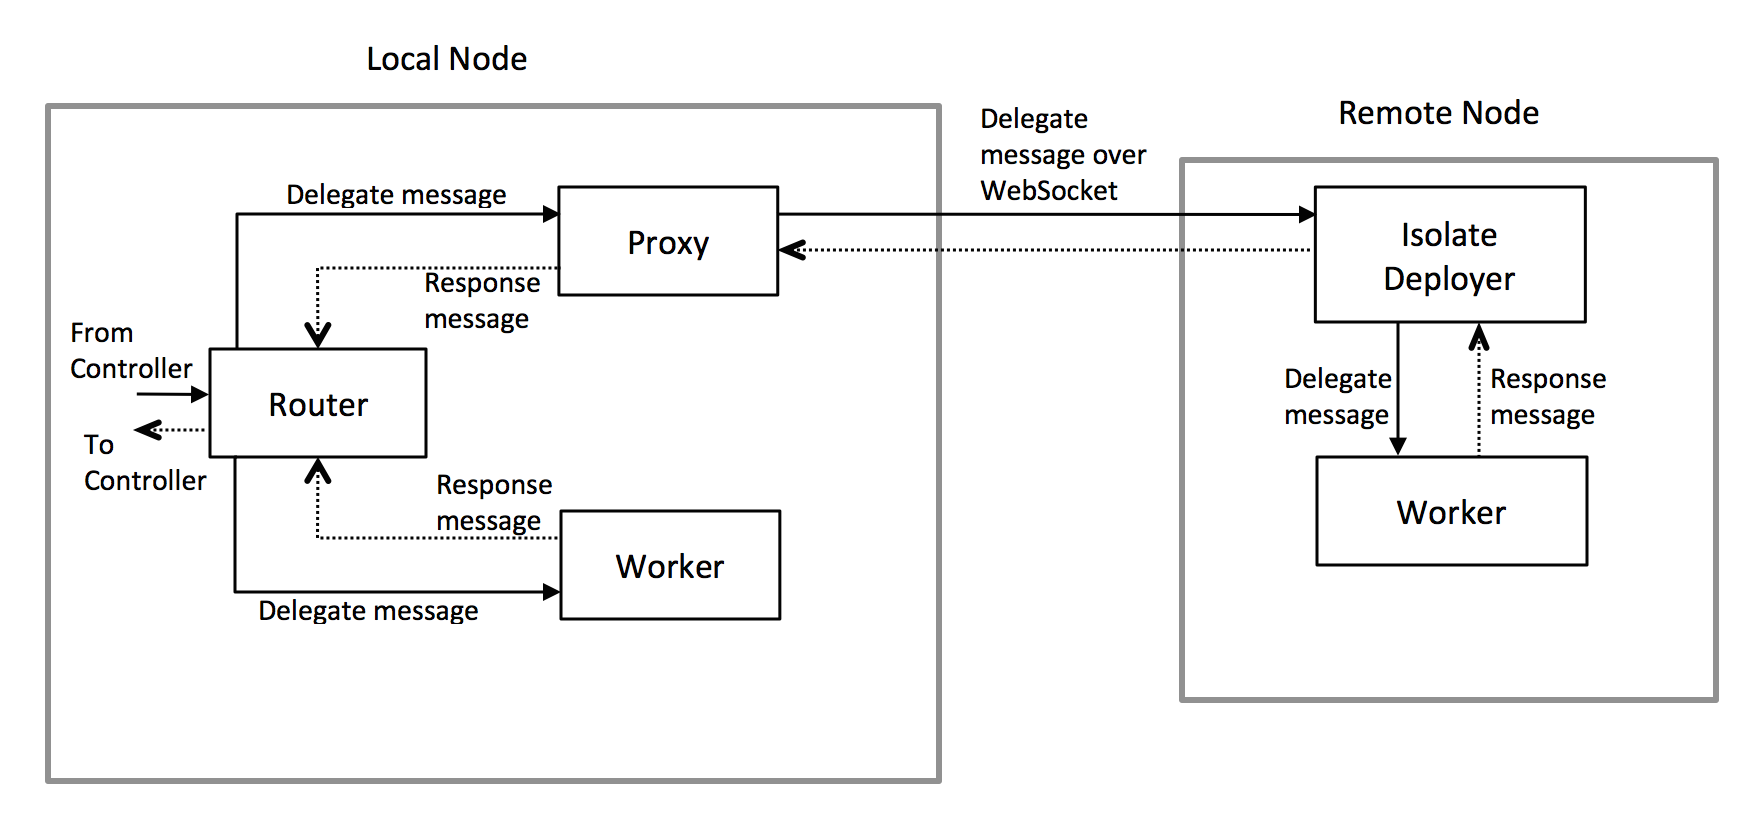
\includegraphics[width=1\textwidth]{figures/proxy}
    \caption[Proxy Worker]{A Proxy Worker}
    \label{fig:proxy}
  \end{figure}

  \subsubsection{FileMonitor}
  \label{subsubsec:fileMonitor}
  A ‘FileMonitor’ is spawned by the controller only if the ‘Hot Deployement’ flag for a worker isolate is set during deployment. The spawned ‘FileMonitor’ monitors the MD5 checksum of the source code from which the Worker isolate is spawned. If a change in the source file is detected, it sends a RESTART message to the controller. The controller forwards the message to the target router to restart the router's worker isolates.

\subsection{The Registry}
\label{subsec:registry}
The isolate registry is a central node where nodes that are running Bootstrappers connect and register. The registry keeps a record of connected nodes, assigns a unique id to each node and queries them about running isolate systems when required. The registry provides a RESTful API and a web interface~\footnote{the web interface can be opted out as it has to be started separately} through which one can have an overview of the full system and manage the deployments of isolate systems as well as individual isolates.

The basic tasks that a registry carries out are:
\begin{itemize}
  \item Bootstrapping an isolate system, during runtime, in a local or remote node
  \item Providing a way to deploy, update or remove an isolate system
  \item Returning information about the deployed isolates by querying the individual isolate systems of a node.
\end{itemize}

  \subsubsection{RESTful API of the Registry}
  \label{subsec:restApi}
  The registry provides a REST API to perform several operations on connected nodes. One can send a ‘GET’ request to the registry to fetch the list of nodes that are connected to the registry. Using an ‘id’ of a node from the replied list, one can deploy an isolate system or add an isolate to an already deployed isolate system by sending an appropriate ‘POST’ request.

  The REST endpoints exposed by a registry are listed in table~\autoref{tab:endpoints}.
  \begin{table}[H]
    \caption[Endpoints exposed by the registry]{List of endpoints exposed by the registry}\label{tab:endpoints}
    \centering
    \begin{tabular}{l l}
      \toprule
        \bf{Method}  & \bf{Endpoint} \\
      \midrule
        GET &  /registry/system/list\\
        GET & /registry/system/\{bootstrapperId\} \\
        POST & /registry/deploy \\
        POST & /registry/system/shutdown \\
      \bottomrule
    \end{tabular}
  \end{table}

\paragraph{A Sample GET and POST Query to Deploy an Isolate System}
\begin{description}
  \item{GET request to fetch a list of connected systems}\\
  Request: ‘GET \url{http://54.77.239.254:8000/registry/system/list}’\\
  Response Status Code: 200 OK\\
  Response Body:
  \begin{lstlisting}[language=json,firstnumber=1]
    [
      {
        "bootstrapperId": "266393094",
        "ip": "54.77.239.244",
        "port": "50189"
      },
      {
        "bootstrapperId": "12133208",
        "ip": "54.77.239.243",
        "port": "50192"
      }
    ]
  \end{lstlisting}

  \item{POST request to deploy an isolate system}\\
  Request: ‘POST \url{http://54.77.239.254:8000/registry/deploy}’\\
  Request Body:
  \begin{lstlisting}[language=json,firstnumber=1]
    {
      "bootstrapperId" : "266393094",
      "action": "action.addIsolate",
      "messageQueuingSystemServer": "ws://54.77.239.200:42043/mqs",
      "isolateSystemName" : "sampleSystem",
      "isolateName" : "consumer",
      "uri" : "http://54.77.239.221/sampleSystem/bin/Consumer.dart",
      "workersPaths" : ["localhost", "ws://54.77.239.243:42042/activator"],
      "routerType" : "random",
      "hotDeployment" : true
    }
  \end{lstlisting}
  Response Status Code: 200 OK
\end{description}

\paragraph{A Sample GET Query to Fetch Details of an Isolate System}
  \begin{description}
    \item{GET request to get details of an isolate system}\\
    Request: ‘GET \url{http://54.77.239.254:8000/registry/system/266393094}’\\
    Response Status Code: 200 OK\\
    Response Body:
    \begin{lstlisting}[language=json,firstnumber=1]
    {
      "sampleSystem": [
        {
          "id": "sampleSystem/consumer",
          "workerUri": "http://54.77.239.221/sampleSystem/bin/Consumer.dart",
          "workersCount": 2,
          "workersPaths": [
            "localhost",
            ws://54.77.239.243:42042/activator"
          ],
          "routerType": "random",
          "hotDeployment": true
        }
      ]
    }
  \end{lstlisting}
  \end{description}

\paragraph{A Sample POST Query to Terminate a Worker Isolate}
  \begin{description}
    \item{POST request to terminate an isolate of an isolate system}\\
    Request: ‘POST \url{http://54.77.239.254:8000/registry/system/shutdown}’\\
    Request Body:
    \begin{lstlisting}[language=json,firstnumber=1]
      {
        "bootstrapperId" : "266393094",
        "isolateSystemName" : "sampleSystem",
        "isolateName" : "consumer"
      }
    \end{lstlisting}
    Response Status Code: 200 OK
  \end{description}

\paragraph{An Example of Terminating an Isolate System}
  \begin{description}
    \item{POST request to terminate an isolate of an isolate system}\\
    Request: ‘POST \url{http://54.77.239.254:8000/registry/system/shutdown}’\\
    Request Body:
    \begin{lstlisting}[language=json,firstnumber=1]
      {
        "bootstrapperId" : "266393094",
        "isolateSystemName" : "sampleSystem"
      }
    \end{lstlisting}
    Response Status Code: 200 OK
  \end{description}

The registry generates all information about isolates and isolate systems “on the fly”. Thus, it does not need to persist any data.

  \subsubsection{The Web Interface for the Registry}
  \label{subsubsection:registryWebInterface}
  Deployment of isolates can also be managed by using a web interface provided by the registry. The web interface must be started up as a separate process than the registry. It internally communicates with the registry using the REST API~[\ref{subsec:restApi}].

  \autoref{fig:registryWebInterface} is a screenshot of the registry web interface showing a list of connected nodes and a list of deployed systems. The interface also shows the details of each isolate. An individual isolate can be terminated using the ‘kill’ button next to an isolate, and an isolate system can be terminated using the ‘shutdown’ button next to the isolate system. To deploy a new worker isolate into a new isolate system, the ‘+’ button may be used, which pops out a form shown in \autoref{fig:registryWebInterface-addisolate}. If the name of an existing isolate system is used when deploying an isolate, the isolate is added to the existing isolate system instead of creating a new isolate system.

\begin{figure}[H]
  \centering
  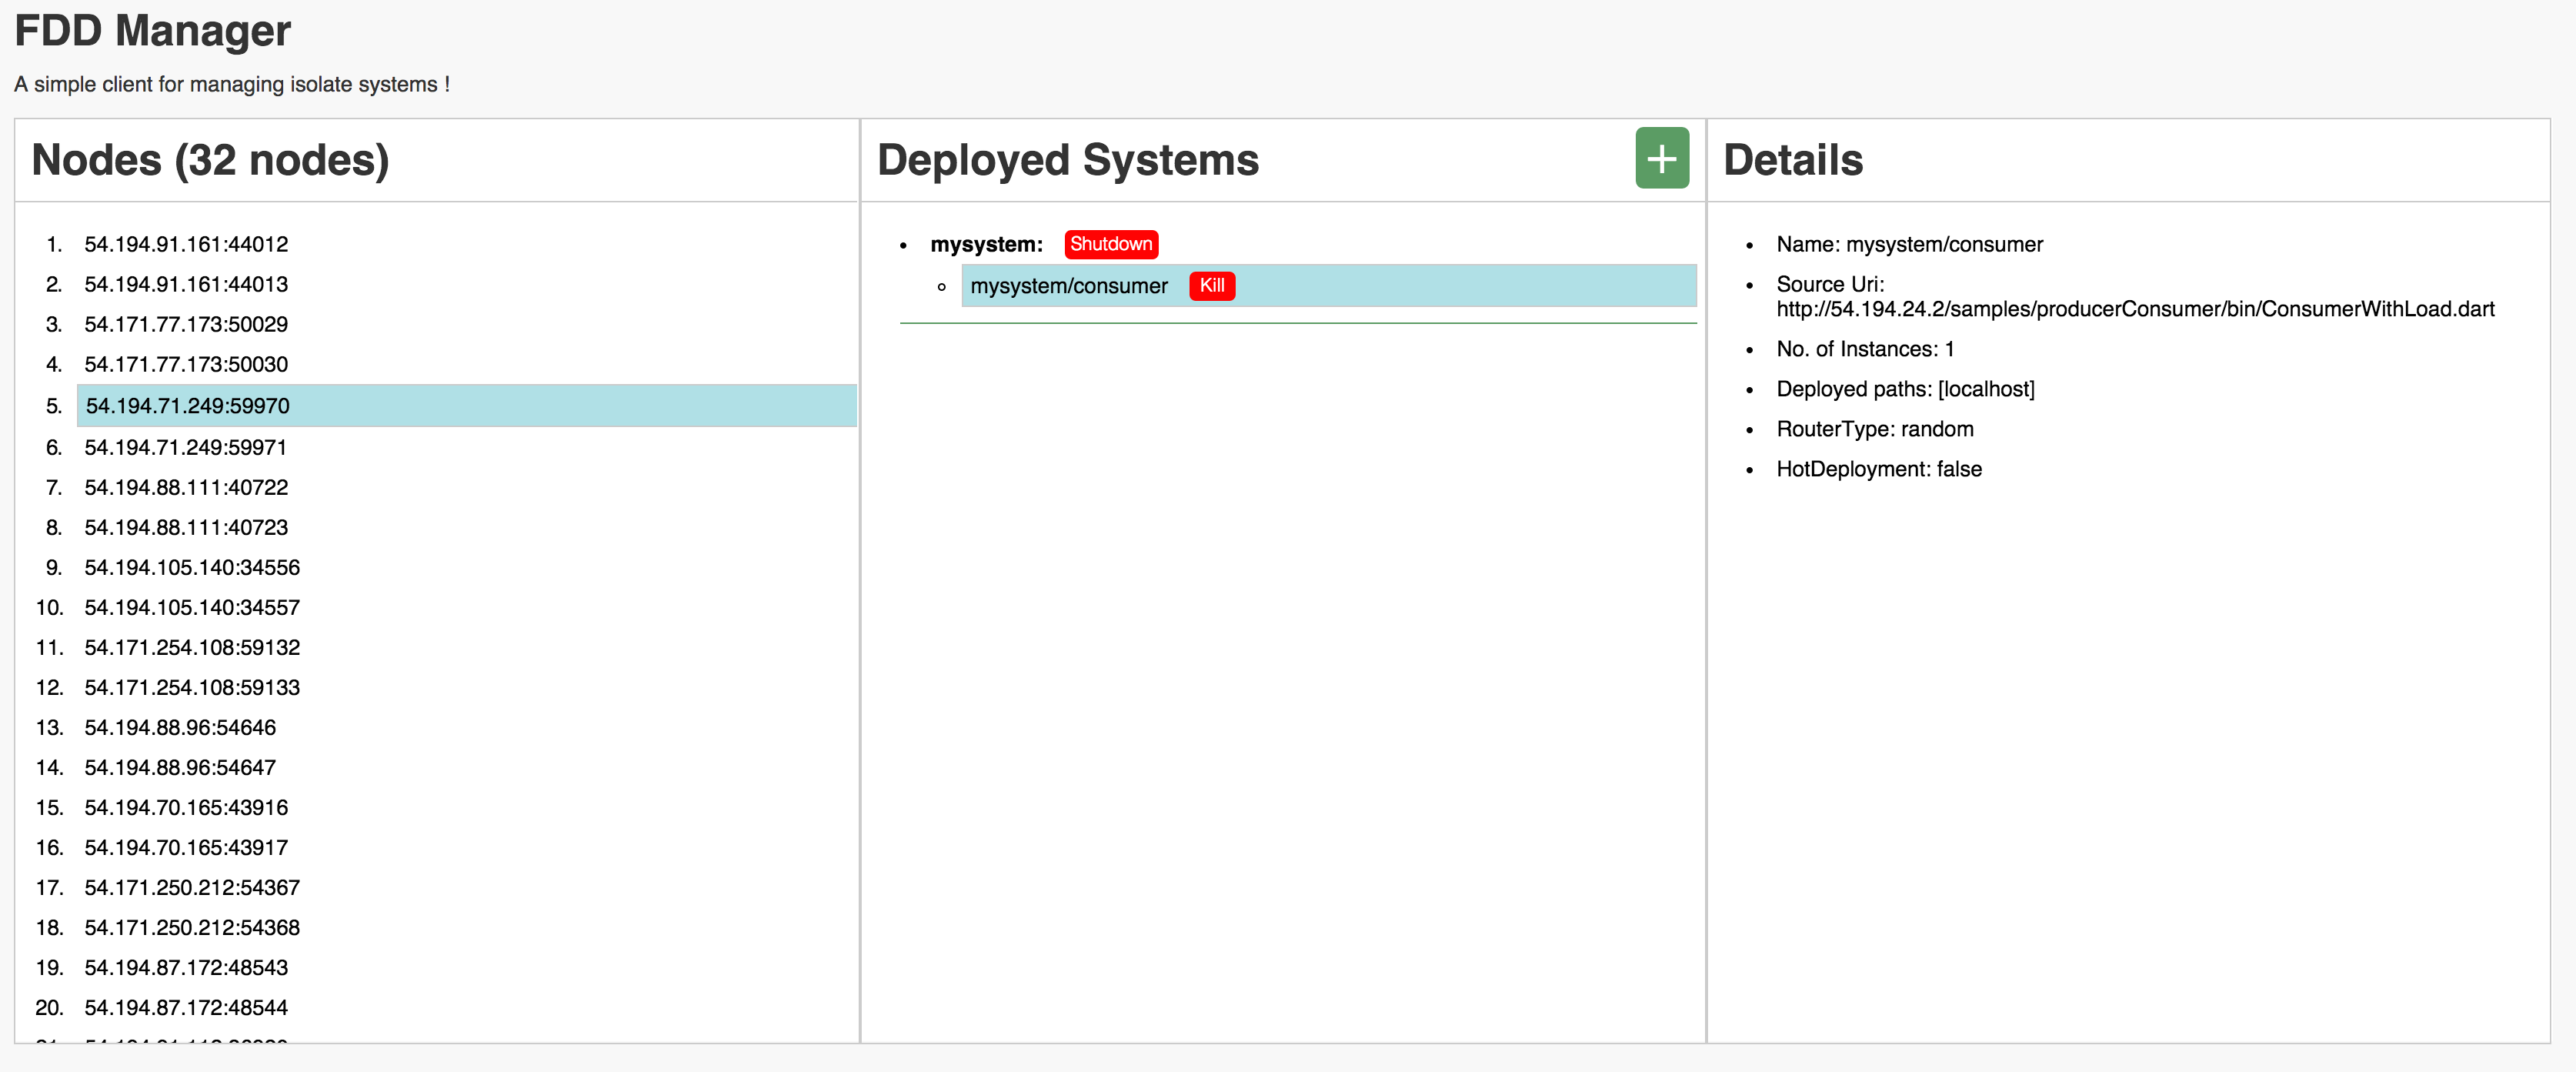
\includegraphics[width=1\textwidth]{figures/webinterface}
  \caption[Web interface of the Registry showing isolate systems and isolates in a node]{Web interface of the Registry showing isolate systems and isolates in a node}
  \label{fig:registryWebInterface}
\end{figure}

\begin{figure}[H]
  \centering  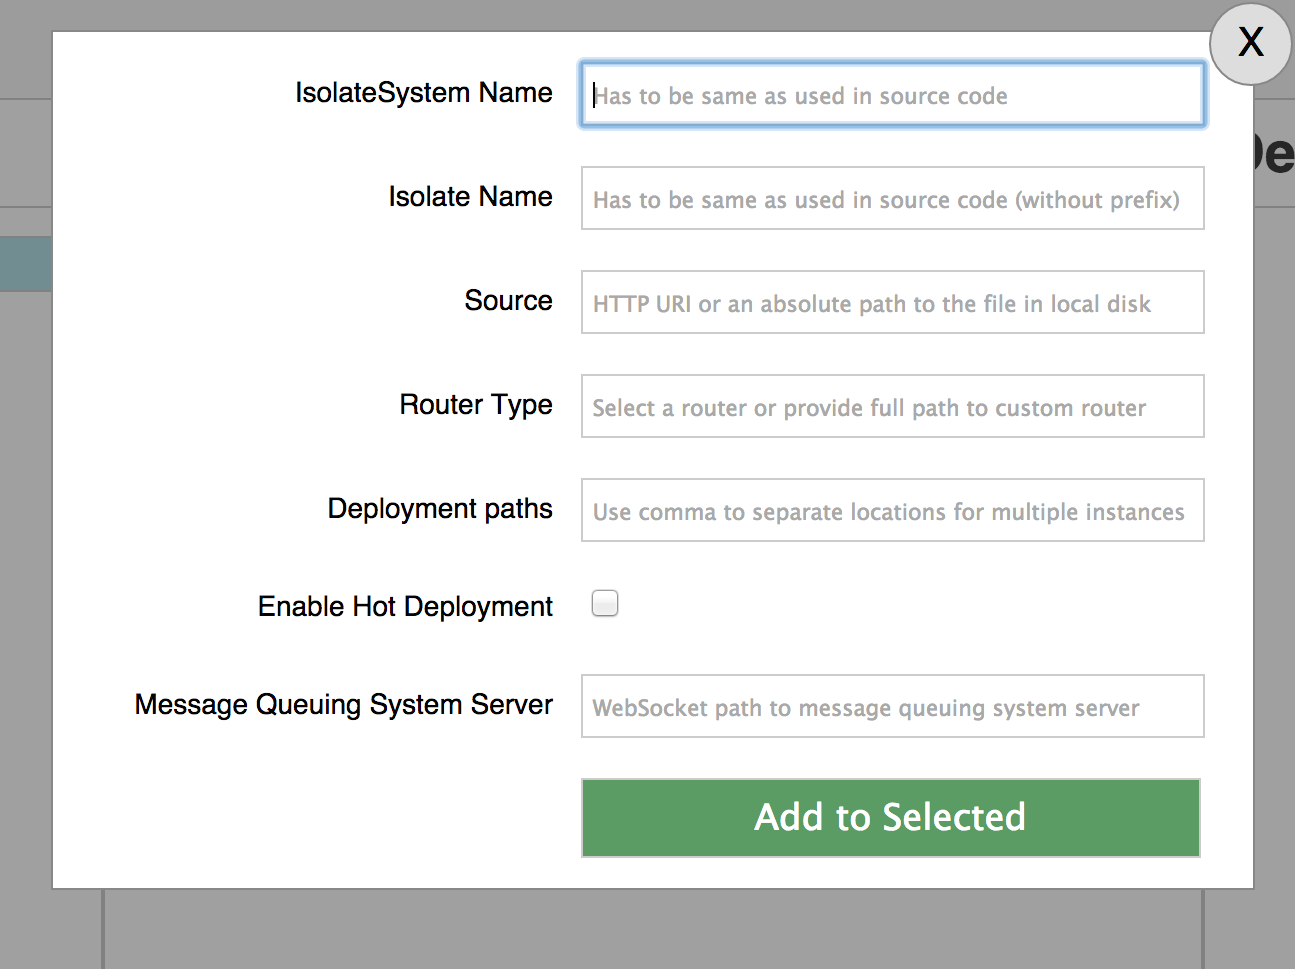
\includegraphics[width=0.8\textwidth]{figures/webinterface-addisolate}
  \caption[Form of the web interface to deploy an isolate]{Form of the web interface to deploy an isolate}
  \label{fig:registryWebInterface-addisolate}
\end{figure}

\subsection{Message Queuing System (MQS)}
\label{subsec:mqs}
  Since the basis of this framework is message passing, a Message Queuing System is an important component. An MQS consists of a top level isolate, an ‘Enqueuer’ and ‘Dequeuers’. The top level isolate fetches messages from a message broker system and dispatches to respective isolates of the isolate system. Whenever a new isolate system starts up, it opens a new WebSocket connection with an MQS through which messages are exchanged. An MQS keeps track of the unique ids of isolate systems so that it can identify the origin of a message.

  If a message should be enqueued, the MQS ignores the unique id and simply forwards the message to an ‘Enqueuer’ isolate. Whereas, if the message is a dequeue request, the MQS forwards the message to a ‘Dequeuer’ isolate along with the unique id of the isolate system. The unique id is required to identify the WebSocket port through which the request arrived. This guarantees that a dequeued message is sent to the correct requester which is required when a cluster of identical isolate systems is running on different nodes.

  An MQS should be started up separately along with command line arguments to connect to a message broker system. The required command line arguments are: IP address, port, username and password to connect to a broker. The ‘prefetchCount’ is an optional argument which defaults to 1, if not provided explicitly. A ‘prefetchCount’ is a Quality of Service header for the message broker system which allows a subscriber of a queue to hold the defined quantity of unacknowledged messages.

Since in Dart\footnote{Dart version 1.7.2} the passing of sockets to isolates is not yet possible, the main isolate has to pipe all input/output data. In this case, an MQS is a top level isolate which handles all incoming and outgoing messages.

  \subsubsection{Enqueuer}
  An enqueuer of an MQS is a separate isolate. An MQS has only one enqueuer, which receives messages from the MQS and sends them to a message broker system (RabbitMQ~[\ref{sec:rabbitmq}]) using the STOMP~[\ref{sec:stomp}] protocol.

  \subsubsection{Dequeuer}
  As opposed to an enqueuer, an MQS maintains a separate dequeuer for each queue of a broker. A queue also corresponds to each router running in an isolate system. Whenever a message arrives from a new isolate, the MQS spawns a new dequeuer isolate. The dequeuer then subscribes to a new message queue in the message broker system using the STOMP~[\ref{sec:stomp}] protocol. If a queue does not exist in the message broker system, the broker automatically creates it.

  If a dequeuer is idle for too long, i.e. if the dequeuer isolate has not received any dequeue requests for a certain interval\footnote{by default the timeout is 10 seconds}, then the MQS terminates the dequeuer isolate for that particular queue. Nevertheless, as soon as the MQS receives a dequeue request, it spawns a new dequeuer if one does not exist yet.

  A dequeuer subscribes for messages from a message broker system with such options that new messages do not arrive to the subscriber unless previously dequeued messages have been acknowledged. This throttles the flow of messages from the message broker system and keeps itself and the isolates from being overwhelmed by a large number of messages and prevents ‘out of memory’ issues.

  Messages in a dequeuer keep arriving as long as there are messages in a queue and they are being acknowledged. The buffered messages of a dequeuer stay unacknowledged unless they are flushed and sent out to the requesting isolate of an isolate system. As soon as a dequeuer acknowledges a message, it receives another message from its message broker.

  \subsubsection{Multiple Instances of the MQS}
  It is possible for an application to have multiple message queuing systems for scaling up. If there are multiple identical isolate systems connected to different instances of an MQS, each MQS will have a dequeuer which subscribes to the same queue. However, a message is dispatched by the message broker system to only one of the dequeuers because it is distributed in a round robin fashion. This ensures that messages are fairly distributed among subscribers.

\subsection{Activator}
  An activator simply starts up two isolates: a ‘System Bootstrapper’ and an ‘Isolate Deployer’. Every node that should be running an Isolate System or become part of an isolate system must be running an activator. An activator requires the WebSocket address of a Registry as a command line argument. Nevertheless, it is also possible to start up a System Bootstrapper and Isolate Deployer separately.

  \subsubsection{System Bootstrapper}
  \label{subsubsec:bootstrapper}
  A System Bootstrapper registers itself to the ‘Registry’ via a WebSocket connection as soon as it is started. The activator forwards the path of a WebSocket to the system bootstrapper. If a system bootstrapper is started separately then the path of the registry should be passed as a command line argument.

  A system bootstrapper is responsible for starting up an instance of an isolate system in a physical node. As it creates an isolate system, it can invoke methods provided by the top level isolate of the isolate system.

  \subsubsection{Isolate Deployer}
  \label{subsubsec:isolateDeployer}
An Isolate Deployer starts up a worker isolate in a node. The worker isolate is spawned without a local isolate system and as a part of an isolate system running in another node. This functionality expands an isolate system beyond a physical system. An isolate system can deploy a number of instances of an isolate in several different nodes.

  An isolate deployer running in a remote machine is able to handle requests from multiple ‘Proxies’ from several isolate systems. Each proxy opens a separate WebSocket channel with an isolate deployer.

\section{Some Key Features}
\subsection{Hot Deployment of Isolates and Isolate Systems}
~\label{subsec:hotDeployment}
The hot deployment feature of the \acrshort{DDE} framework allows source code of an isolate to reside in a remote repository. For instance, source code of an isolate can reside in a git repository hosted in GitHub. When new code is committed to the repository, it gets immediately picked up by the application and the change is reflected without restarting.

  After a node is bootstrapped, changes like adding, updating or removing isolates in an isolate system can take place. In such cases, isolates are killed and redeployed when they have finished processing and are idle. A dedicated isolate ‘FileMonitor’~[\autoref{subsubsec:fileMonitor}] monitors changes in the code repository. When a change is detected, the ‘FileMonitor’ isolate sends a RESTART message along with the target router to notify the controller. The controller takes care of pushing the message to the relevant router, and the router takes care of terminating and re-spawning the worker isolates.

  This hot deployment capability improves the availability of an application. When there is any change in a component of an application, the whole application does not need to be re-deployed. Instead, only a set of isolates that should be updated are restarted at runtime. This increases overall up-time of an application and keeps other components working even during modifications.

\subsection{Migration of Isolates and Isolate Systems}
  Migration of isolates is the relocation of worker isolates or an isolate system during runtime. This requires killing one or more worker isolates in one node and spawning them in another node. The concept of hot deployment and migration brings enormous possibilities for a distributed system. Some of them are:

\begin{itemize}

  \item Migration of isolates allows an application to adapt to deployment topologies in an easy way. This allows an application to respond to varying load and traffic.

  \item Related and dependent isolates can be migrated to the same server, if it is evident that it improves performance of the entire system.

  \item In case of imminent critical system failure, migration of worker isolates during runtime can make the application survive the failure.

\end{itemize}

\subsection{Remote Isolates}
\label{subsec:remoteIsolate}
  The current isolate implementation in Dart\footnote{Dart version 1.7.2} cannot communicate with other isolates over a network. Worker isolates in this framework have the ability to communicate with isolates that are running in a remote node. The communication underneath is taken care of by the framework so developers do not have to worry if an isolate is remotely or locally spawned. Two isolates running in different virtual machines can still belong to the same logical isolate system. Having remote isolates provides the \acrshort{DDE} framework with clustering, high availability, greater scalability and isolate migration.

\section{Typical Message Flow in the System}
The \acrshort{DDE} framework is based on the ‘fire-and-forget’ principle of message sending. \autoref{fig:enqueueMessage} shows a simple message flow while enqueuing a message and \autoref{fig:dequeueMessage} shows the process of dequeuing a message.

  A message is serialized to JSON string before sending via a SendPort of an isolate and deserialized after receiving from a ReceivePort.

\begin{figure}[H]
  \centering
  \tiny
\begin{sequencediagram}
\newinst[0.5]{w}{Worker (Entry point)}
\newinst[0.5]{r}{Router}
\newinst[0.5]{c}{Controller}
\newinst[0.5]{s}{Isolate System}
\newinst[0.5]{m}{MQS}
\newinst[0.5]{e}{Enqueuer}
\newinst[0.5]{rab}{RabbitMQ}

  \mess{w}{serialize and send message}{r}
  \mess{r}{delegate message}{c}
  \mess{c}{delegate message}{s}
  \mess{s}{delegate message}{m}
  \mess{m}{delegate message}{e}
  \mess{e}{enqueue message}{rab}

\end{sequencediagram}
  \caption{Enqueuing a message}
  \label{fig:enqueueMessage}
\end{figure}
\normalsize

\begin{figure}[H]
  \centering
  \tiny
\begin{sequencediagram}
\newinst[0.5]{w}{Idle Worker}
\newinst[0.5]{r}{Router}
\newinst[0.5]{c}{Controller}
\newinst[0.5]{s}{Isolate System}
\newinst[0.5]{m}{MQS}
\newinst[0.5]{deq}{Dequeuer}
\newinst[0.5]{rab}{RabbitMQ}

  \mess{w}{done}{r}
  \mess{r}{dequeue request}{c}
  \mess{c}{dequeue request}{s}
  \mess{s}{dequeue request}{m}
  \mess{m}{dequeue request}{deq}
  \mess{deq}{acknowledge buffered messages}{rab}
  \mess{deq}{flush buffered messages}{m}
  \mess{rab}{new messages}{deq}
  \mess{m}{dequeued messages}{s}
  \mess{s}{dequeued messages}{c}
  \mess{c}{dequeued messages}{r}
  \mess{r}{route dequeued messages}{w}
\end{sequencediagram}
  \caption{Dequeuing a message}
  \label{fig:dequeueMessage}
\end{figure}
\normalsize

\subsection{Sample Message formats}

\subsubsection{A Message Sent Through Different Components While Enqueuing}

\begin{description}

\item Original Message:
\begin{lstlisting}[language=json,numbers=none]
"Test"
\end{lstlisting}

\item Worker:
\begin{lstlisting}[language=json,numbers=none]
{senderType: senderType.worker, id: sampleSystem/producer/88f52440-5060-11e4-f396-97cebb949945, action: action.send, payload: {sender: sampleSystem/producer, to: sampleSystem/consumer, message: Test, replyTo: null}}
\end{lstlisting}

\item Router:
\begin{lstlisting}[language=json,numbers=none]
{senderType: senderType.router, id: sampleSystem/producer, action: action.send, payload: {sender: sampleSystem/producer, to: sampleSystem/consumer, message: Test, replyTo: null\}\}
\end{lstlisting}

\item Controller:
\begin{lstlisting}[language=json,numbers=none]
{senderType: senderType.controller, id: sampleSystem/producer, action: action.send, payload: {sender: sampleSystem/producer, to: sampleSystem/consumer, message: Test, replyTo: null\}\}
\end{lstlisting}

\item Top level isolate:
\begin{lstlisting}[language=json,numbers=none]
{targetQueue: sampleSystem.consumer, action: action.enqueue, payload: {sender: sampleSystem/producer, message: Test, replyTo: null}}
\end{lstlisting}

\item Message Queuing System:
\begin{lstlisting}[language=json,numbers=none]
{topic: sampleSystem.consumer, action: action.enqueue, payload: {sender: sampleSystem/producer, message: Test, replyTo: null}}
\end{lstlisting}

\item Enqueuer:
\begin{lstlisting}[language=json,numbers=none]
  {sender: sampleSystem/producer, message: Test, replyTo: null}
\end{lstlisting}
\end{description}

\subsubsection{Sample Format of a Message Sent at Different Components While Dequeuing}
\begin{description}
\item Dequeuer:
\begin{lstlisting}[language=json,numbers=none]
{"sender":"mysystem/producer","message":"Test","replyTo":null}
\end{lstlisting}

\item Message Queuing System:
\begin{lstlisting}[language=json,numbers=none]
{senderType: senderType.dequeuer, topic: mysystem.consumer, payload: {sender: mysystem/producer, message: Test, replyTo: null}
\end{lstlisting}

\item Top level isolate of isolate system:
\begin{lstlisting}[language=json,numbers=none]
{senderType: senderType.isolate_system, id: mysystem, action: action.none, payload: {to: mysystem/consumer, message: {sender: mysystem/producer, message: Test, replyTo: null}}}
\end{lstlisting}

\item Controller:
\begin{lstlisting}[language=json,numbers=none]
{senderType: senderType.controller, id: controller, action: action.none, payload: {to: mysystem/consumer, message: {sender: mysystem/producer, message: Test, replyTo: null}}}
\end{lstlisting}

\item Router:
\begin{lstlisting}[language=json,numbers=none]
{senderType: senderType.router, id: mysystem/consumer, action: action.none, payload: {sender: mysystem/producer, message: Test, replyTo: null}}
\end{lstlisting}

\item Worker:
\begin{lstlisting}[language=json,numbers=none]
"Test"
\end{lstlisting}

\end{description}

\subsection{Some Implementation Overview}
\label{subsec:implementationOverview}
  Some insight about the implementation of selected functions of the framework:

  \begin{description}
    \item How \emph{send} works?\\
      When a worker isolate sends a message using the \emph{send} function, the message is encapsulated with further information about the sender and receiver. The encapsulated message is forwarded to a spawner isolate, which is a router. The router again forwards it to a controller which again forwards to a top level isolate. Then the top level isolate adds another level of encapsulation and headers to the message so that an MQS knows the destination queue.

      If a worker isolate is expecting to consume another message after sending one, it should send a PULL Request, which can be performed by invoking the \emph{done} function.

      \item \label{itm:askWorking}How \emph{ask} works?\\
    The \emph{ask} function has a subtle differences from the \emph{send} function. The \emph{ask} function should be used when the sender of a message expects a reply message. The abstract Worker class adds the full path of an isolate along with the unique id of the isolate when an ‘ask’ message is constructed. This is to make sure that the response from a target isolate reaches this particular instance of an isolate. When a router receives a message with a complete address (name along with its unique id) of a worker isolate, it routes the message to a specific worker regardless of its routing algorithm. If a worker isolate with the given unique id is not found in the router's list of worker isolates, then the message is simply discarded. This is possible when isolates have been restarted or for some reason isolates were killed.

    \item How \emph{reply} works?\\
    The \emph{reply} function is simply a convenience for a developer. The \emph{reply} function invokes the \emph{send} function with the sender’s address as the target isolate. If the message contains a ‘replyTo’ header then the message is sent to the address contained in ‘replyTo’ instead of the original sender. The \emph{reply} function can be used for replying to messages for both the \emph{send} and \emph{ask} cases.

    \item \label{itm:killWorking} How ‘KILL’ works?\\
    This is a special control message sent to isolates and isolate systems to shutdown themselves. If a KILL message is sent to a worker isolate, the message is enqueued to the end of its queue. Messages arriving after a KILL message are not sent to the worker isolate and are buffered until the isolate is restarted. The messages are delegated to a worker isolate only after its spawning is complete.

    When a worker isolate finishes processing queued messages and encounters a KILL message, the isolate closes its ReceivePort\footnote{A Worker Isolate receives message from Router via a ReceivePort} and stays idle. After sometime it gets garbage collected by the VM. Sometimes the garbage collector cannot clean up an isolate and a memory leak occurs. As a workaround, a custom ‘Exception’ is thrown deliberately by an isolate to terminate itself. The exception is thrown only after the isolate closes all ports. This workaround forcefully terminates the isolate and releases memory occupied by the isolate.

    The abstract Worker class provides the \emph{beforeKill()} method, which can be overridden to perform custom operations before terminating an isolate.

    \item How ‘RESTART’ works?\\
    Restarting an isolate is basically a combined process of killing an isolate and spawning it up again. However, after issuing a KILL message, messages may continue coming from a controller to a router while restarting. These messages are buffered in the router itself. The buffered messages are flushed and sent out once the Worker isolates are spawned. For instance, when the ‘Hot Deployment’~\autoref{subsec:hotDeployment} feature is enabled, if the source code of an isolate is modified and saved, each of the isolates that a router has spawned gets restarted. During which messages that arrive after a RESTART message are buffered in the router.

    \item How shutting down an isolate system works?\\
    An isolate system that is running in a node can be shutdown via the web interface of the registry or by sending a POST request to the registry. When a request to shutdown an isolate system is received, the isolate system closes all its ports including the ReceivePort, SendPort and the WebSocket connection with the MQS. After that a forceful shutdown is carried out by throwing a custom Exception. This is a workaround to free up the consumed memory because the feature to immediately terminate an isolate is yet to be implemented in Dart.
  \end{description}

\subsection{Clustering}
  Clustering can be achieved in the \acrshort{DDE} framework at several levels:
  \begin{itemize}
  \item By deploying worker isolates in several remote nodes. i.e. taking advantage of the concept of ‘Remote Isolates’~[\autoref{subsec:remoteIsolate}].
  \item By deploying replicas of an isolate system in different nodes. An isolate system with same name can exist in another node even though they connect to the same MQS.
  \item The Message Queuing System itself can also be replicated where replicas of the isolate system may connect to different instance MQS.
  \item Since several instances of RabbitMQ~[\autoref{sec:rabbitmq}] can form a logical group sharing common configuration, properties, users, queues etc., a cluster of message brokers can be formed. This allows Message Queuing Systems to connect to the different members of a cluster.
  \end{itemize}

  \autoref{fig:cluster} is an example of a cluster formed by deploying a worker isolate ‘A’ across multiple isolate systems. The isolate systems are connected to separate instances of the MQS. Each MQS is connected to a separate node of the RabbitMQ cluster.

\begin{figure}[H]
  \centering
  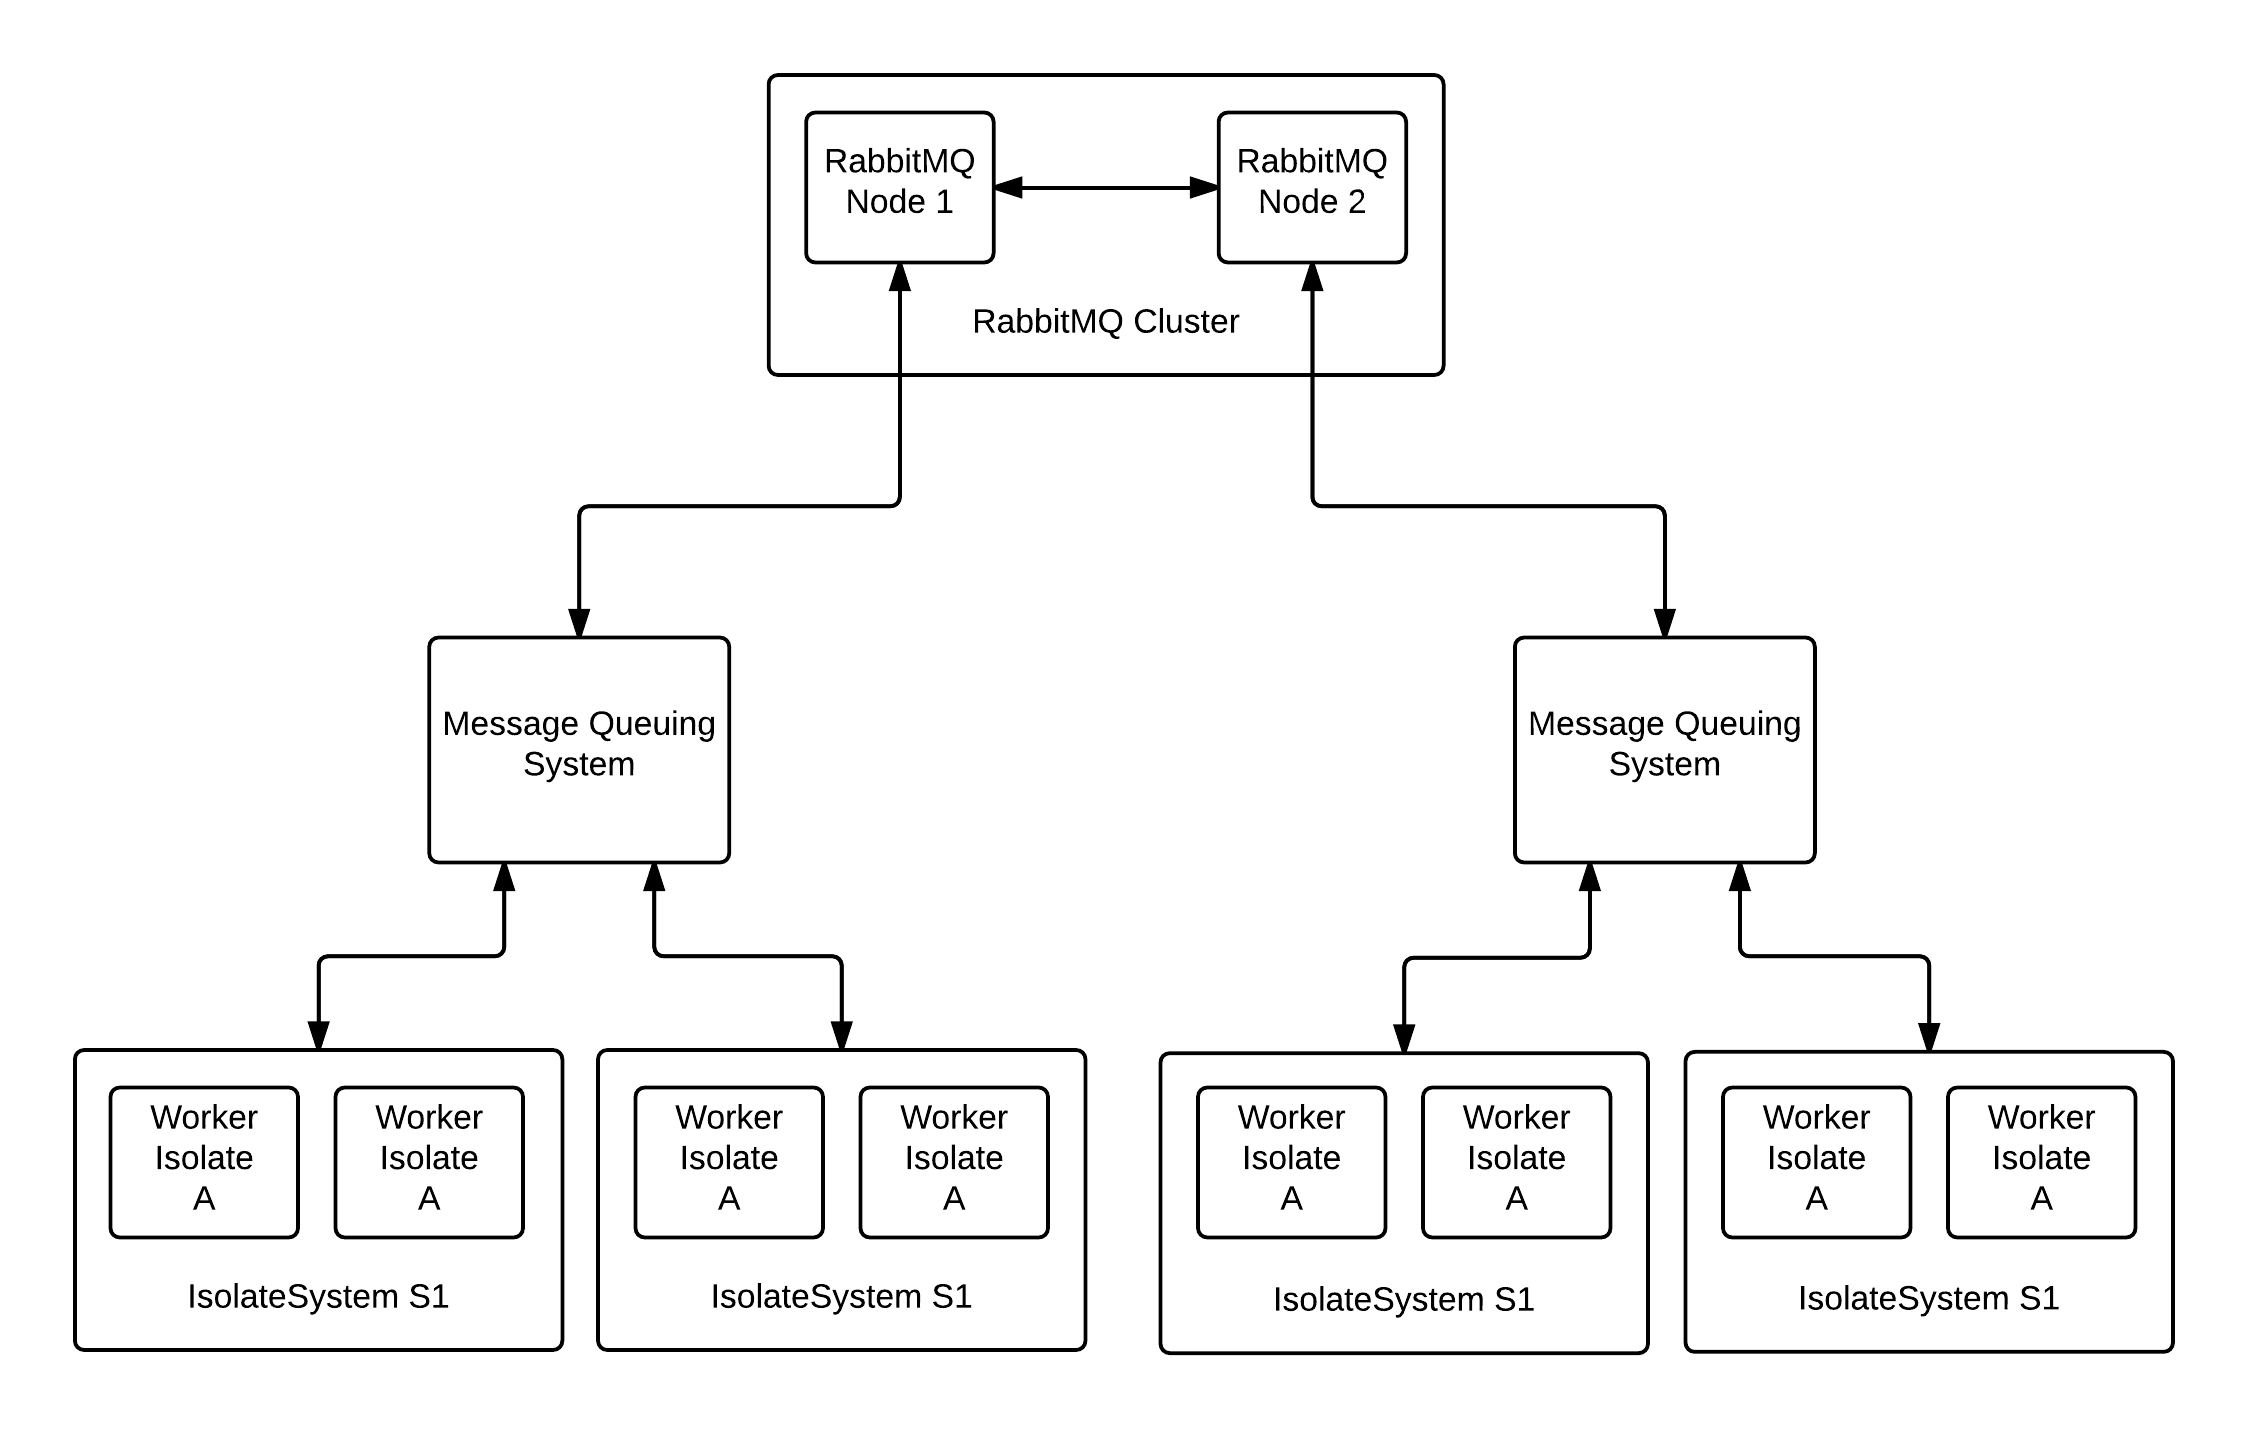
\includegraphics[width=1\textwidth]{figures/cluster}
  \caption[Forming a cluster in \acrshort{DDE} Framework]{Forming a cluster in \acrshort{DDE} Framework}
  \label{fig:cluster}
\end{figure}

\section{Dart Libraries Used in the \acrshort{DDE} Framework}
\autoref{tab:libraries} is the list of third-party libraries that are used by the \acrshort{DDE} framework. All of these libraries are open source and available in Dart's pub.

\begin{table}[htsb]
  \caption[Dependent libraries of the framework]{List of libraries directly used by the framework}\label{tab:libraries}
  \centering
  \begin{tabular}{l l}
    \toprule
      \bf{Library} & \bf{URL} \\
    \midrule
      path &  \url{https://pub.dartlang.org/packages/path}\\
      uuid &  \url{https://pub.dartlang.org/packages/uuid}\\
      crypto &  \url{https://pub.dartlang.org/packages/crypto}\\
      stomp &  \url{https://pub.dartlang.org/packages/stomp}\\
    \bottomrule
  \end{tabular}
\end{table}

\section{A Sample Implementation of Worker Using \acrshort{DDE} Framework}
\autoref{lst:sampleWorker} is an example implementation of a worker isolate for the \acrshort{DDE} framework. The \emph{main()} function is the entry point of the isolate, which is invoked when this isolate is spawned by a router. The class \emph{Consumer} overrides the function \emph{onReceive()}, which is called for each incoming message.

  The example shown here prints a message if an ‘action’
 set in the \emph{message} variable is “print”. If the ‘action’ set in the \emph{message} variable is “send\textunderscore{}back” then the Worker isolate sends the message back to sender.

\begin{lstlisting}[language=java,firstnumber=1, caption=A sample Worker isolate that can be deployed in the framework, label=lst:sampleWorker]
    import 'dart:isolate';
    import 'package:isolatesystem/worker/Worker.dart';

    main(List<String> args, SendPort sendPort) {
      Consumer printerIsolate = new Consumer(args, sendPort);
    }

    class Consumer extends Worker {
      Consumer(List<String> args, SendPort sendPort) : super(args, sendPort);

      @override
      onReceive(message) {
        switch(message['action']) {
          case "print":
            print("message['content']");
            break;
          case "send_back":
            reply(message['content']);
            break;
        }
        done();
      }
    }

\end{lstlisting}
